\section{Chapitre 2 - La m�thode de Monte-Carlo}


Voici le code :
\lstinputlisting[language=Scilab]{02-Integration-complement/Scripts-Scilab/MonteCarlo-simple.sci}

\begin{cor}$ $\\
\begin{center}
	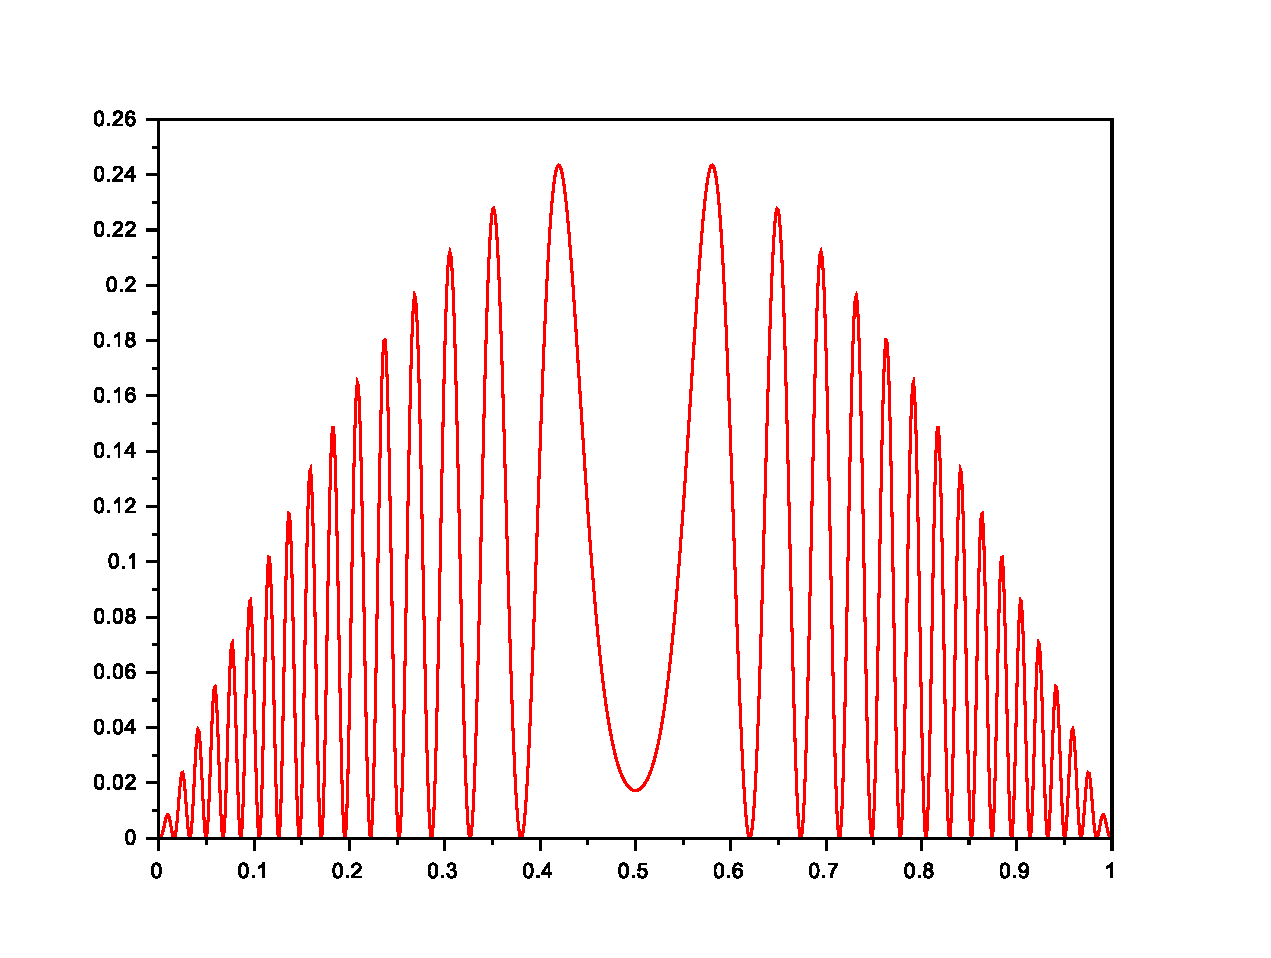
\includegraphics[width=0.4\textwidth]{02-Integration-complement/Scripts-Scilab/fonction.pdf}
\end{center}
\end{cor}

\begin{cor}
On obtient le r�sultat suivant :
\begin{lstlisting}
-->[r,e]=rect(f,0,1,100)
 e  = 0.0000155708600156623245  
 r  = 0.0805132891947099027519
\end{lstlisting}
\end{cor}

\begin{cor}
On obtient le r�sultat suivant
\begin{lstlisting}
-->MonteCarlo(f,0,1,1000)
 ans  = 0.0827886208728949440916 
\end{lstlisting}
\begin{center}
	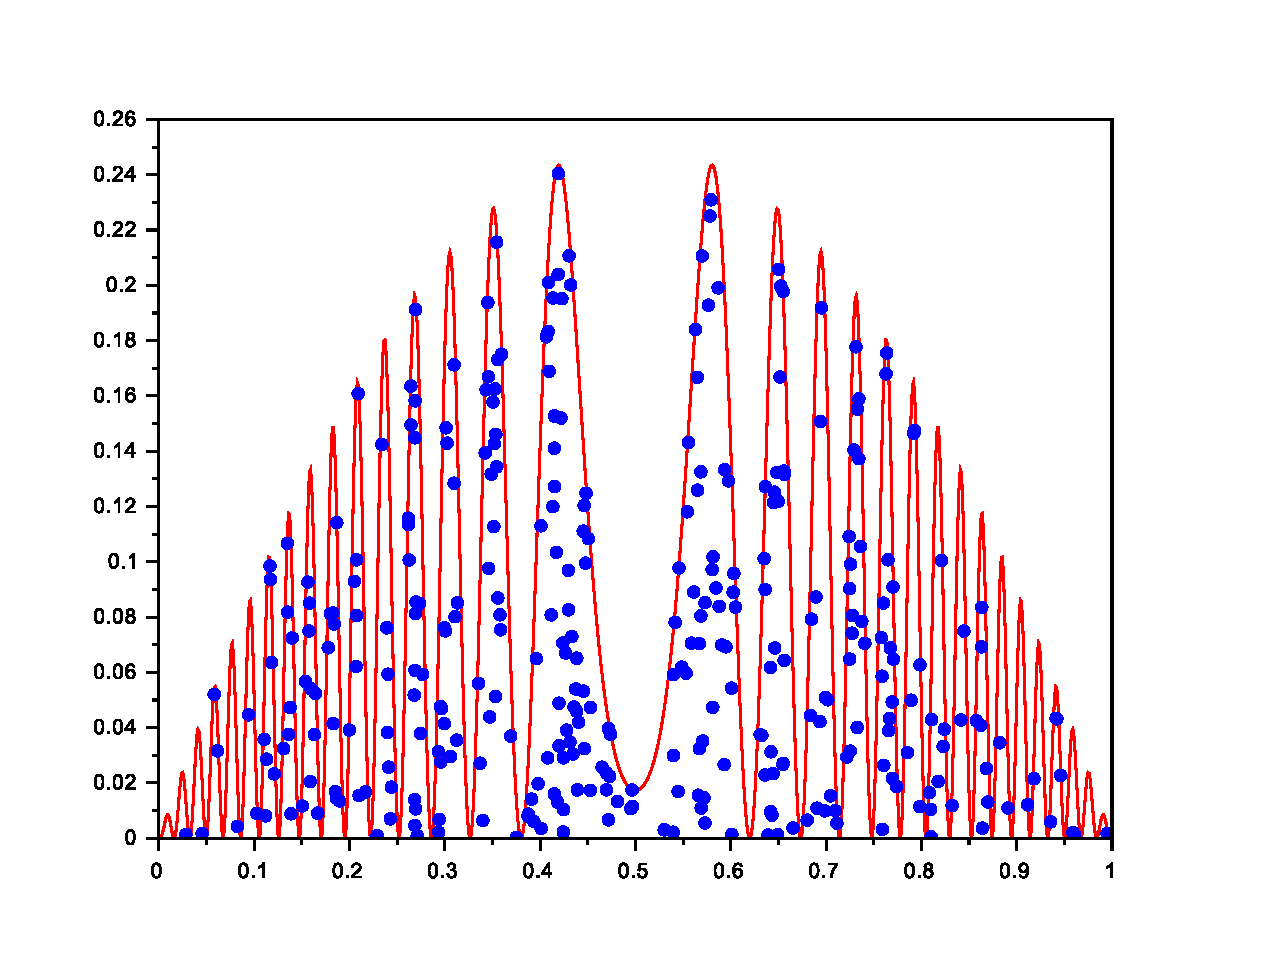
\includegraphics[width=0.48\textwidth]{02-Integration-complement/Scripts-Scilab/MonteCarlo1.pdf}
\end{center}
On peut n�anmoins remarquer que la m�thode n'est pas tr�s stable car si on r�p�te on essaye � nouveau \textbf{le m�me programme}, on obtient un r�sultat tout � fait diff�rent :
\begin{lstlisting}
-->MonteCarlo(f,0,1,1000)
 ans  = 0.0771882141667873389324
\end{lstlisting}
\end{cor}



\begin{cor}
On obtient le r�sultat suivant :
\begin{lstlisting}
-->MonteCarlo2(f,0,1,1000)
 ans  = 0.0779629211010469530541
\end{lstlisting}
ou
\begin{lstlisting}
-->MonteCarlo2(f,0,1,500)
 ans  = 0.0822603994629290680152
\end{lstlisting}
\begin{center}
	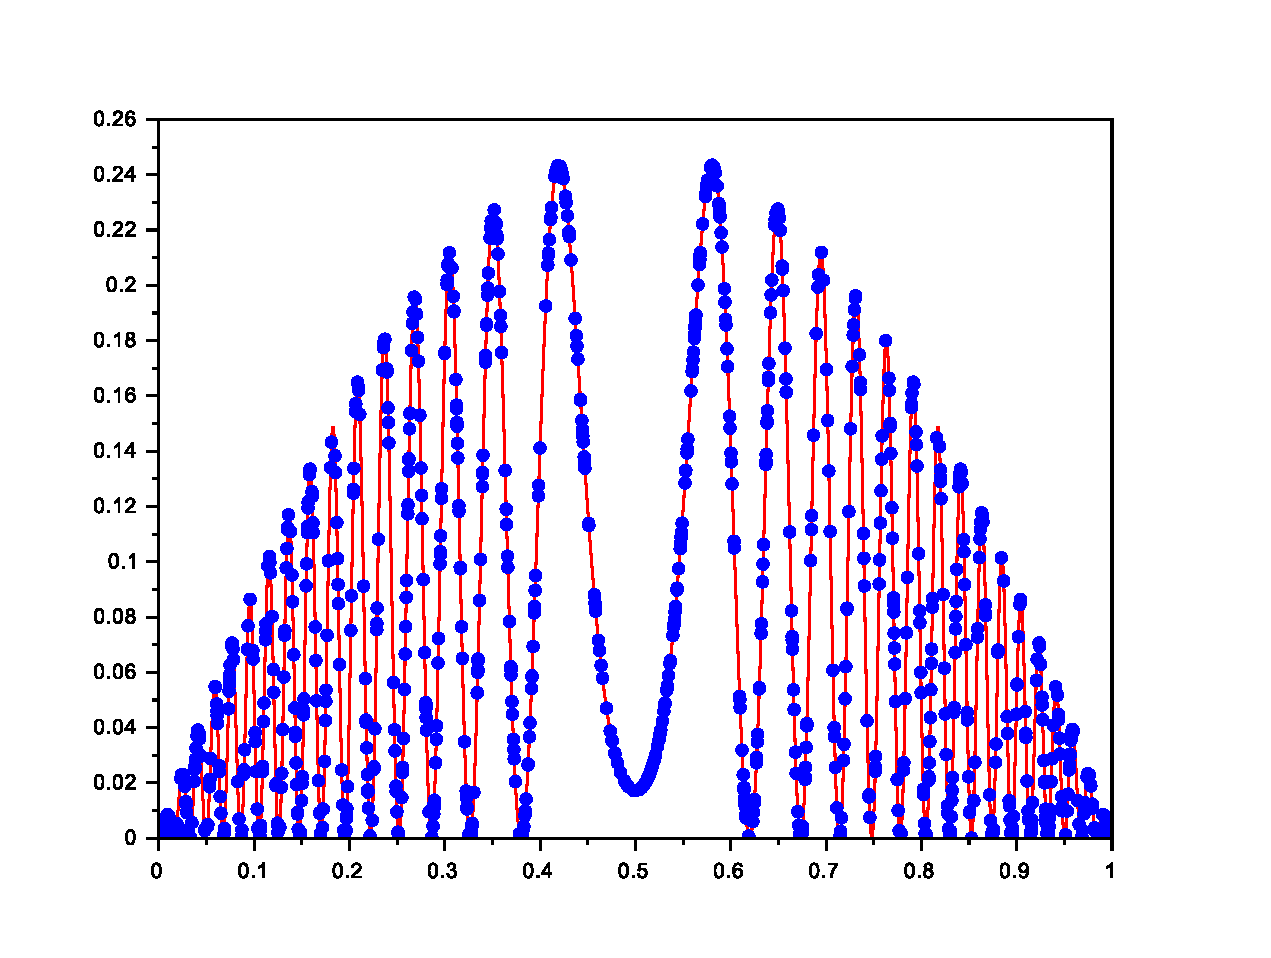
\includegraphics[width=0.48\textwidth]{02-Integration-complement/Scripts-Scilab/MonteCarlo2.pdf}
\end{center}
\end{cor}

Le programme propos� est tr�s int�ressant car il est tr�s visuel. On voit au fur et � mesure les nouveaux points choisis au hasard. Le probl�me c'est que Scilab n'arr�te pas de faire des va et vient entre le calcul d'un point et son affichage ce qui ralentie l'ex�cution du programme. Il est donc pr�f�rable d'opter pour une version o� on calcule tous les points que l'on garde en m�moire dans une matrice, puis d'afficher tous ces points. Gagnant nettement en rapidit�, on pourra demander � calculer beaucoup plus de points. Le r�sultat sera alors plus fiable.\\

Voici notre nouveau programme avec un chronom�tre pour comparer avec la m�thode pr�c�dente :\\
\lstinputlisting[language=Scilab]{02-Integration-complement/Scripts-Scilab/MonteCarlo-matriciel.sci}

Les r�sultats sont les suivants :\\
\begin{tabularx}{\textwidth}{XX}
\begin{center}
	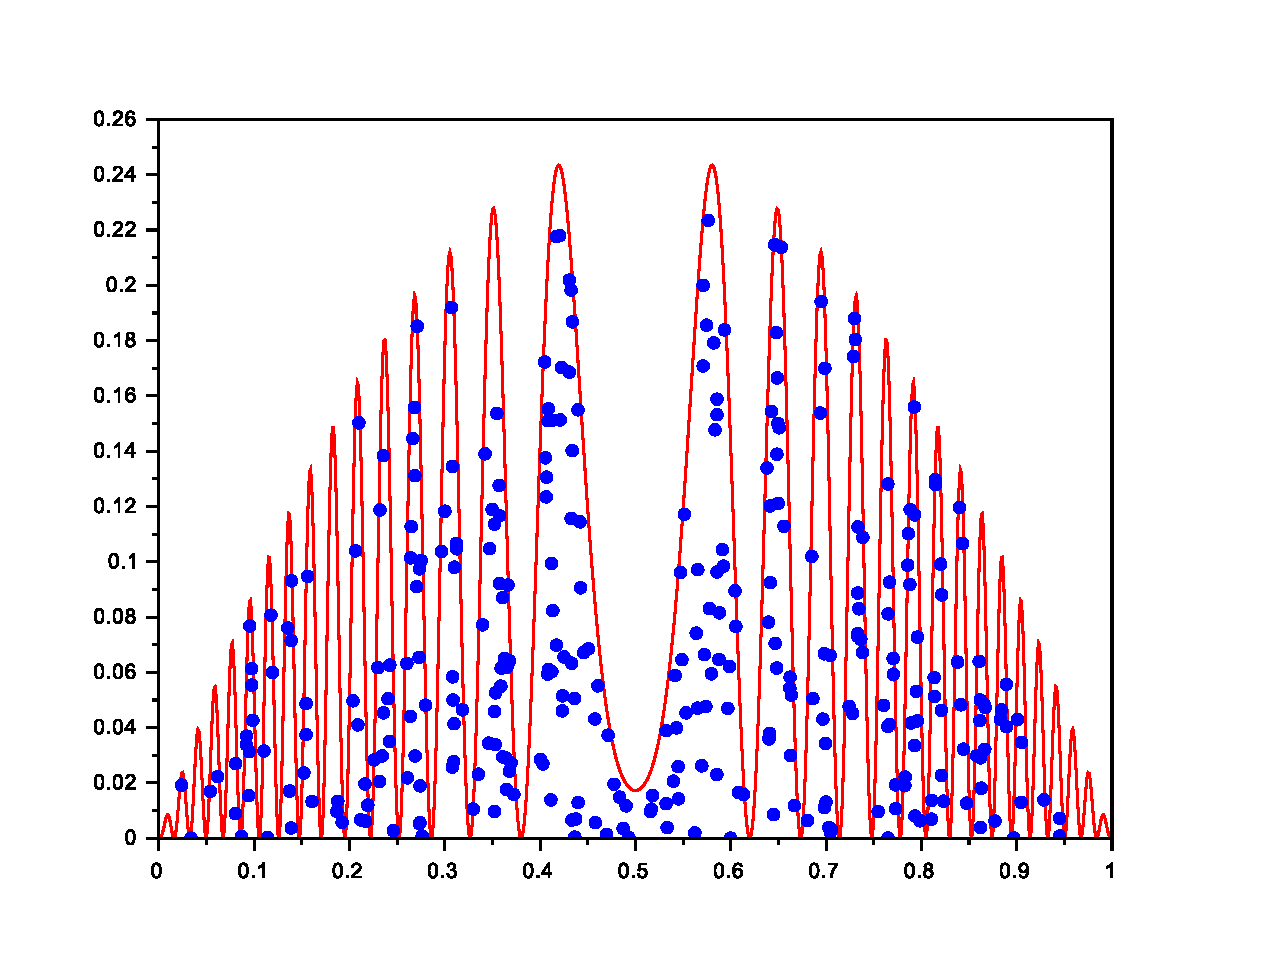
\includegraphics[width=0.48\textwidth]{02-Integration-complement/Scripts-Scilab/MonteCarlo1-matriciel-1000.pdf}
\end{center}
Avec 1~000 points, on obtient \newline
le r�sultat de 0.0793796776604816234357\newline
en 0.0469999999999999307221 seconde.
&
\begin{center}
	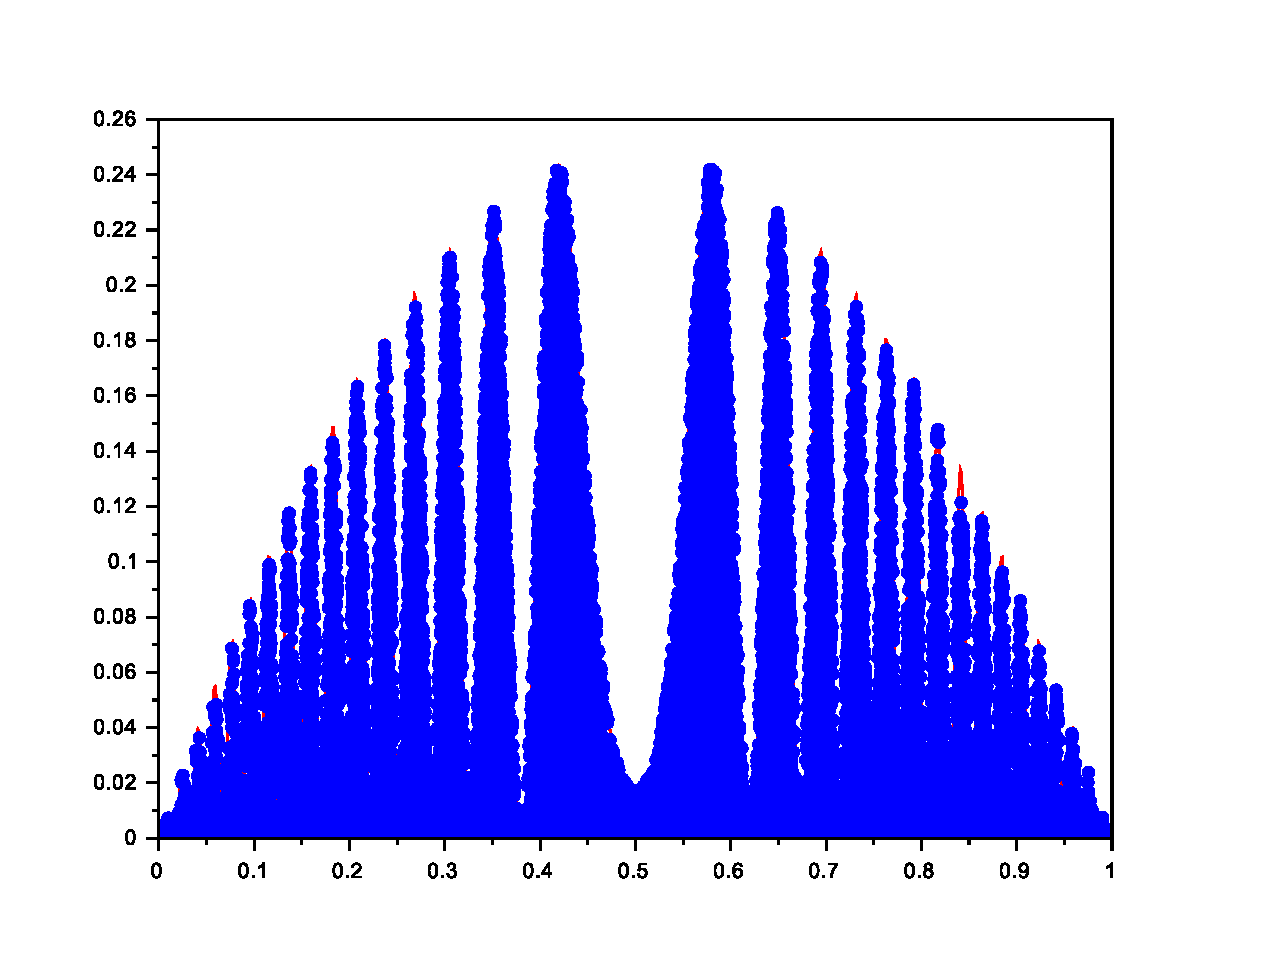
\includegraphics[width=0.48\textwidth]{02-Integration-complement/Scripts-Scilab/MonteCarlo1-matriciel-50000.pdf}
\end{center}
Avec 50~000 points, on obtient\newline
le r�sultat de 0.0807676045398213332538\newline
en 3.326 secondes.
\\
\end{tabularx}

\medskip

A comparer avec la premi�re version qui nous donne un r�sultat pour 1~000 points en 13.276999999999999246825 secondes (mais on a une animation). Je n'ose pas essayer avec les 50~000 points...\\
...\\
Mais 5~000 points se fait en un peu moins de 167 secondes et 10~000 points en 556 secondes\footnote{En r�alit� j'ai bien essay� les 50~000 points mais mon ordinateur s'est mis en veille avant d'avoir termin� son calcul ...}.